\chapter{Material and Methods}

\textbf{SARS-CoV 2 genome data set}

We create a dataset of 360 genetic sequences from December 2019 to March 8 2020, obtained from publicly available data on GISAID \cite{GISAID} (accessed on November 2020). We follow the Nextstrain workflow for the curation of the dataset \cite{nextstrain}. Sequences with incomplete collection date, less than 27.000 bases in length or with more than 3.000 unknown bases are omitted. Also, sequences from known clusters of transmission or from the same patient are excluded from the analysis. The resulting dataset of x \todo{look number of seqs} sequences is aligned with MAFFT. The beggining and the end of the alignment are masked respectively by 100 and 50 sequences as well as sites  13402, 24389 and 24390, identified by Nextstrain as prone to sequencing errors.

To focus on the early dynamics in Europe we select sequences from China, origin of the epidemic, France and Germany, the European countries with the earliest cases, and Italy and Spain, the European countries with the biggest outbreaks in March. To take into account the dynamics in other regions of Europe we include a group of 50 sequences from other European countries. We limit our sample of Chinese genomes to sequences until January 23, the starting date of the lockdown in Hubei. 

Due to the large (and unprecendented) number of available genetic sequences for SARS-CoV-2, we need to subsample the alignment. Each sequence is subsampled with a probability of having a reported case in that country the day of sample collection, inversely weigted by the probability of having a sequence in GISAID that day from the country. With this subsampling protocol, we aim to get a constant sampling proportion accross the full period for each country. 

This dataset of genetic sequences is the main source of information for our phylodynamic analysis. The goal is to infer the phylogenetic tree, i.e. the evolutionary tree-shaped relationship among the sequences, together with the epidemiological transmission parameters that gave rise to it. These parameters are defined within a population dynamic model and will inform us about the epidemic in the population that the sequences come from.

\textbf{The multitype birth death model}

To study the early dynamics of SARS-CoV-2 in the European countries, we use a simplified version of the multitype birth-death model described in \cite{Kuhnert2016}, following the analysis in \cite{Nadeau2020}. Birth death models are compartmental population models with high flexibility that describe the process of epidemiological transmission. The stochastic formulation of these models are used in phylodynamic analyses \cite{Stadler2012}. In the multitype version, we consider a structured population in types or subpopulations with characteristic within-subpopulation dynamics and migrations between them. In our case, the subpopulations are the different locations of the samples.

The process starts with one infected host in one of the subpopulations, e.g in subpopulation $i$, who can infect another individual at rate $\lambda_i$, become uninfectious at rate $\mu_i$ by death or recovery, migrate to another deme $j$ at rate $m_{ij}$ or be sequenced at rate $\psi_i$ to become part of the phylogenectic tree. This process depicts the full transmission dynamics and specifically, the generation of the phylogenetic tree that we observed from our sequence data. 

Under this model, we are able to compute the likelihood of the multitype birth-death parameters for a given tree. This likelihood is derived in \cite{Kuhnert} by considering the probability of an individual evolved as observed in the tree. This derivation is analogous to the work in Stadler and Bonhoeffer (2013), which is based on ideas from (Maddison et al. 2007)

We parameterize our model in terms of the effective reproductive number $R_i = \frac{\lambda_i}{\mu_i + \psi_i}$, a key value in epidemic control and understanding, the rate of becoming uninfectious $\delta_i = \mu_i + \psi_i$ and the probability of and individual to be sequenced $s_i = \frac{\psi_i}{\mu_i + \psi_i}$.\\

\textbf{Epidemic trajectories and structured trees}

We will refer to the full sequence of transmissions, recoveries/deaths, migrations and sampling events as an epidemic trajectory. One set of sequences, and therefore one phylogenetic tree, is the product of one epidemic trajectory. Moreover, the tree represents a fraction of the events in the epidemic trajectory, those that involve the sampled individuals. In epidemiology, we aim to learn about the true epidemic trajectory since we usually have incomplete information caused by unreported cases or unknown transmission chains.

From the sequences metadata, we know the location of the tree tips. However, if we know the epidemic trajectory we also know the location of the lineage at any point in time in the tree. We will refer to the phylogenies with ancentral locations mapped onto the tree as structured trees \cite{Vaughan2014}. In Fig \ref{fig:epitrajs} we show the epidemic trajectories corresponding to two different subpopulations and the structured tree of a set of samples. The change of ancestral location, represented by a change in color from blue to red in the tree, is caused by a migration event from one subpopulation to the other depicted in the epidemic trajectories.

\begin{figure}[h]
    \centering
    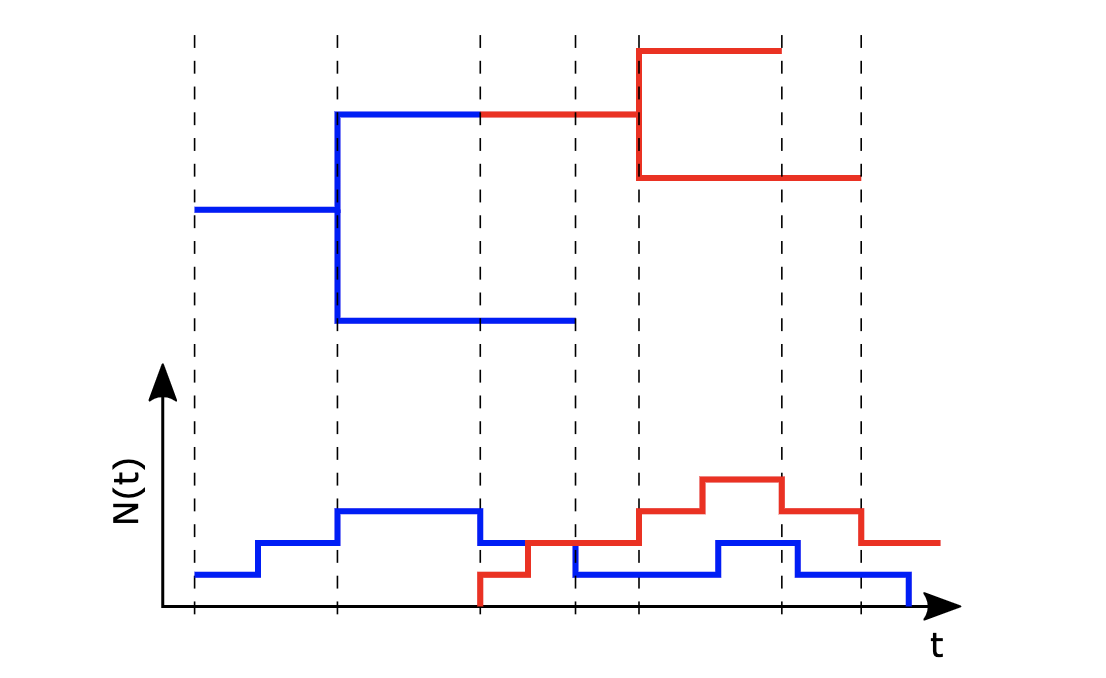
\includegraphics[width=\textwidth]{figures/epitrajs.png}
    \caption{Example of structured tree (up) and epidemic trajectories (bottom) for two types. The horizontal axis represents time, and for the epidemic trajectories the vertical axis is the population size N(t). Figure from Tim Vaughan.}
    \label{fig:epitrajs}
\end{figure}

\textbf{BDMM-Prime Inference}

We want to infer the epidemic trajectories under the multitype birth-death model fit to SARS-CoV-2 early epidemics in Europe. In order to do this, we have to estimate the overall posterior distribution of the structured tree $\mathcal{T}_c$, the epidemic trajectory $\mathcal{E}$, the substitution model parameters $\theta$ and the multi-type birth death parameters $\eta$. This posterior probability can be expressed with Bayes' formula as:

\begin{equation}
P(\mathcal{T}_c, \mathcal{E}, \theta, \eta | A ) = \frac{P(A | \mathcal{T}_c, \mathcal{E}, \theta, \eta ) P(\mathcal{T}_c, \mathcal{E}, \theta, \eta)}{P(A)}
\label{eq:posterior1}
\end{equation}

where A is the sequence alignment.

We make the following independence assumptions:

\begin{align}
P(A | \mathcal{T}_c, \mathcal{E}, \theta, \eta ) &= P(A | \mathcal{T},\theta )\\
P(\mathcal{T}_c, \mathcal{E}, \theta, \eta) &= P(\mathcal{T}_c|\mathcal{T}, \eta) P(\mathcal{E}|\mathcal{T}_c, \eta) P(\mathcal{T} | \eta ) P(\theta) P(\eta)
\label{eq:assumptions}
\end{align}


Where $\mathcal{T}$ is the rooted time tree without ancestral locations. Thus,

\begin{equation}
P(\mathcal{T}_c, \mathcal{E}, \theta, \eta | A) = P(\mathcal{T}_c|\mathcal{T}, \eta) P(\mathcal{E}|\mathcal{T}_c, \eta) \frac{P(A | \mathcal{T}, \theta) P(\mathcal{T} | \eta) P(\theta) P(\eta)}{P(A)}
\label{eq:posterior2}
\end{equation}

We use a MCMC Metropolis hastings algorithm implemented in BEAST 2 to smaple from this distribution. No marginal likelihood P(A) calculation.

The factorization of the posterior probability in this way allow us to use the fast solution and The third term in equation \ref{eq:posterior2} is the standard posterior probability infer in BDMM. SO we can use the fast solutions from ..
{}
The tree likelihood $P(A | \mathcal{T},\theta )$ is the probability of the sequence alignment and can be efficiently evaluated using Felsenstein’s pruning algorithm (Felsenstein, 1981). The tree prior, $P(\mathcal{T} | \eta)$ also called phylodynamic likelihood is derived from the multitype birth-death model. $P(\theta)$ and $P(\eta)$ represent our prior belief in the distribution of the population and substitution model parameters. 

While it is possible to do it in the same step \cite{epiestim} it is very slow and computationally expensive. With these two step analyses implmented in BDMM-Prime \cite{bdmm-primegit} the epidemic trajectory inference has almost no overcost and we obtain the same result.


From the phylogenetic tree and the phylodynamics parameters we use Stochastic mapping to infer the ancestral traits and then to infer the epidemic trajectories.

$P(Tc | T, P)$

New method to infer epidemic trajectories!!

$P(E | Tc, P)$

Stochastic mapping of ancestral traits

Read paper and tim presentation

Stochastic mapping of epidemic trajectories

From the phylogenie with ancestral locations and the set of phylodynamic parameters we can simulate epidemic trajectories using an algorithm similar to Gillespie (with tau leaping and particle filtering? the subsampling). And most improtant, we can compute the probability of that specific trajectory given those parrameters and tree. 

$P(E|Tc, P)$

Any trajectories without the events that are respresent in the tree has probability 0, so to avoid the simualtion of this trajectories, no time effcieint, we will enforce the events that arer represented in the tree (and will include a weigth). Also to avoid low probabilities trajectories, we will importance subsample one trajectory after a certain time of simulation according to the weigths detemrined by its probabilities. 



\textbf{Incorporating travel data}

To incorporatet travel data in the model we have use a GLM model described in Lemey et al 2009. We use a generalized linear model to describe the migration matrix KxK, where the rpedictors are the number of dayly flight from one country to another from EUROSTATS, the average distance between the centrroids of the country and the population sizes from origin and destinations. The predictors are log transformed, we add a pseudocount to make them all positive, and standardized as described in ..

$mij = c exp(\sum_{i = 1}^p \delta_i \beta_i xij)$

The coefficients beta describe the effect size of the predictors in the migrations rate and the delta coefficients act as a model selection variables, taking 0-1 values including orr not that specific predictor in the model.

GLM predictos data

EUROSTAT, countries considers. Distance and population datasets.


\textbf{Model specifications and priors}

The time range of our analysis lasts from the origin of SARS-CoV-2 to March 8, when the first European lockdown in the Lombardy region started. This period in the European countries we expect an unimpeded spread of the virus that could be described by a constant R0 particular to each deme. However, the migration rates could have changed during these months due to the increase public awareness, so we will consider a different migration rate for origin to 23 jan, 23 jan to end of february and 1 to 8 of March. We assume a constant sampling proportion different for each of the demes, to account for difference in the sequencing efforts. The becoming uninfectious rate we will fixed in 36.5, assuming that one individual is infectious for a exponential time distirbuted with mean 10.

Since we focus on the early epidemic outbreak, we expect un unimpeded spread of the virus that can be described by the exponential growth of the infected population. Thus, we assume a constant basic reproductive number $R_0$ for each of the European countries. We assume that the $R_0$ for China changes two times during this period, on January 23 and March 1.

We focus on a special scenario, where only the early epidemic outbreak, i.e. exponential growth of the infected population, is being considered. We can simplify the model to a constant rate birth-death process, where we assume no significant decrease in the number of susceptibles over time \cite{TanjaBonhoeffer2014}


We use bayesian inference and Metropolis Hasting Monte Carlo algorith to infer our phylodynamics parameters and phylogeneit tree. We use the following priors

Clock rate and substitution model. Fixed to 8x10-4, HKY 4 gamma categories with priors...
BDMM-Prime epi parameterization:
R0
Become uninfectious rate
Sampling rates
Migration rates


R0 constant except for China (and Italy? maybe not in the main analysis).

Prior Log Normal (0.8, 0.5) Median 2.2, 95IQR 0.8 to 5.9.
(Lai A. 2020 prior log normal (0,1) median 1.0 0.1-7.10)

- Main analysis: We fix China R0 to 2.7 (23 jan) 1.3 (10 feb) 0.8
- Use a decreasing paramater as Sarah with migration rate? But then we would need to add sequences.
- Or instead of fixing it we can put a strong informative prior.
- Allow Italy R0 to change March 1.


Meta-analyses R0:

R0 in China (3.14,95\%CI,2.40–4.09).\cite{Billah2020}

R0value 2.90 (2.32, 3.63
 2.9 (95\% CI: 2.1–4.5)\cite{Park2020}


Periods:
until 23 jan R0 2.9 
23 jan - 10 feb 1.1 dashboard cevo
10 feb - 8 mar 0.43 dashboard cevo



Become uninfectious rate same for all demes, fixed to 36.5.
Migrations among demes, 3 epochs.
Sampling proportion 0 before first sample. Upperbounded by number of cases.

Implementation BEAST 2.6.3 and BDMM-Prime package.
We run 5 chains of 10e7 iterations witth different seeds.


\textbf{Processing of epidemic trajectories}
In our case, for each set of parameters and tree we will simulate 10000 trajectories with an epsilon of 0.3 and select one of them with importance sampling.
We have one trtajectory for each step in the MCMC. We subsampled x. 

\textbf{Data availability}
GISAID data table.

\textbf{Code availability and analyses reproducibility}
All the code is availables at ...
We have implement the full workflow with Snakemake so its fully reproducible.

